\documentclass[1p]{elsarticle_modified}
%\bibliographystyle{elsarticle-num}

%\usepackage[colorlinks]{hyperref}
%\usepackage{abbrmath_seonhwa} %\Abb, \Ascr, \Acal ,\Abf, \Afrak
\usepackage{amsfonts}
\usepackage{amssymb}
\usepackage{amsmath}
\usepackage{amsthm}
\usepackage{scalefnt}
\usepackage{amsbsy}
\usepackage{kotex}
\usepackage{caption}
\usepackage{subfig}
\usepackage{color}
\usepackage{graphicx}
\usepackage{xcolor} %% white, black, red, green, blue, cyan, magenta, yellow
\usepackage{float}
\usepackage{setspace}
\usepackage{hyperref}

\usepackage{tikz}
\usetikzlibrary{arrows}

\usepackage{multirow}
\usepackage{array} % fixed length table
\usepackage{hhline}

%%%%%%%%%%%%%%%%%%%%%
\makeatletter
\renewcommand*\env@matrix[1][\arraystretch]{%
	\edef\arraystretch{#1}%
	\hskip -\arraycolsep
	\let\@ifnextchar\new@ifnextchar
	\array{*\c@MaxMatrixCols c}}
\makeatother %https://tex.stackexchange.com/questions/14071/how-can-i-increase-the-line-spacing-in-a-matrix
%%%%%%%%%%%%%%%

\usepackage[normalem]{ulem}

\newcommand{\msout}[1]{\ifmmode\text{\sout{\ensuremath{#1}}}\else\sout{#1}\fi}
%SOURCE: \msout is \stkout macro in https://tex.stackexchange.com/questions/20609/strikeout-in-math-mode

\newcommand{\cancel}[1]{
	\ifmmode
	{\color{red}\msout{#1}}
	\else
	{\color{red}\sout{#1}}
	\fi
}

\newcommand{\add}[1]{
	{\color{blue}\uwave{#1}}
}

\newcommand{\replace}[2]{
	\ifmmode
	{\color{red}\msout{#1}}{\color{blue}\uwave{#2}}
	\else
	{\color{red}\sout{#1}}{\color{blue}\uwave{#2}}
	\fi
}

\newcommand{\Sol}{\mathcal{S}} %segment
\newcommand{\D}{D} %diagram
\newcommand{\A}{\mathcal{A}} %arc


%%%%%%%%%%%%%%%%%%%%%%%%%%%%%5 test

\def\sl{\operatorname{\textup{SL}}(2,\Cbb)}
\def\psl{\operatorname{\textup{PSL}}(2,\Cbb)}
\def\quan{\mkern 1mu \triangleright \mkern 1mu}

\theoremstyle{definition}
\newtheorem{thm}{Theorem}[section]
\newtheorem{prop}[thm]{Proposition}
\newtheorem{lem}[thm]{Lemma}
\newtheorem{ques}[thm]{Question}
\newtheorem{cor}[thm]{Corollary}
\newtheorem{defn}[thm]{Definition}
\newtheorem{exam}[thm]{Example}
\newtheorem{rmk}[thm]{Remark}
\newtheorem{alg}[thm]{Algorithm}

\newcommand{\I}{\sqrt{-1}}
\begin{document}

%\begin{frontmatter}
%
%\title{Boundary parabolic representations of knots up to 8 crossings}
%
%%% Group authors per affiliation:
%\author{Yunhi Cho} 
%\address{Department of Mathematics, University of Seoul, Seoul, Korea}
%\ead{yhcho@uos.ac.kr}
%
%
%\author{Seonhwa Kim} %\fnref{s_kim}}
%\address{Center for Geometry and Physics, Institute for Basic Science, Pohang, 37673, Korea}
%\ead{ryeona17@ibs.re.kr}
%
%\author{Hyuk Kim}
%\address{Department of Mathematical Sciences, Seoul National University, Seoul 08826, Korea}
%\ead{hyukkim@snu.ac.kr}
%
%\author{Seokbeom Yoon}
%\address{Department of Mathematical Sciences, Seoul National University, Seoul, 08826,  Korea}
%\ead{sbyoon15@snu.ac.kr}
%
%\begin{abstract}
%We find all boundary parabolic representation of knots up to 8 crossings.
%
%\end{abstract}
%\begin{keyword}
%    \MSC[2010] 57M25 
%\end{keyword}
%
%\end{frontmatter}

%\linenumbers
%\tableofcontents
%
\newcommand\colored[1]{\textcolor{white}{\rule[-0.35ex]{0.8em}{1.4ex}}\kern-0.8em\color{red} #1}%
%\newcommand\colored[1]{\textcolor{white}{ #1}\kern-2.17ex	\textcolor{white}{ #1}\kern-1.81ex	\textcolor{white}{ #1}\kern-2.15ex\color{red}#1	}

{\Large $\underline{12a_{1207}~(K12a_{1207})}$}

\setlength{\tabcolsep}{10pt}
\renewcommand{\arraystretch}{1.6}
\vspace{1cm}\begin{tabular}{m{100pt}>{\centering\arraybackslash}m{274pt}}
\multirow{5}{120pt}{
	\centering
	\includegraphics[width=112pt]{../../../GIT/diagram.site/Diagrams/png/2008_12a_1207.png}\\
\ \ \ A knot diagram\footnotemark}&
\allowdisplaybreaks
\textbf{Linearized knot diagam} \\
\cline{2-2}
 &
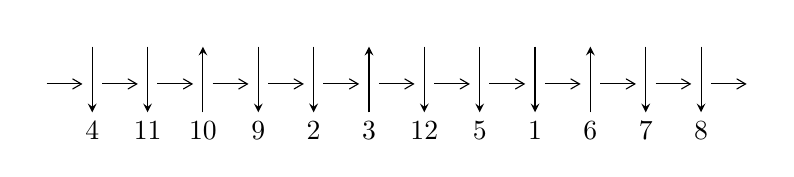
\begin{tikzpicture}[x=20pt, y=17pt]
	% nodes
	\node (C0) at (0, 0) {};
	\node (C1) at (1, 0) {};
	\node (C1U) at (1, +1) {};
	\node (C1D) at (1, -1) {4};

	\node (C2) at (2, 0) {};
	\node (C2U) at (2, +1) {};
	\node (C2D) at (2, -1) {11};

	\node (C3) at (3, 0) {};
	\node (C3U) at (3, +1) {};
	\node (C3D) at (3, -1) {10};

	\node (C4) at (4, 0) {};
	\node (C4U) at (4, +1) {};
	\node (C4D) at (4, -1) {9};

	\node (C5) at (5, 0) {};
	\node (C5U) at (5, +1) {};
	\node (C5D) at (5, -1) {2};

	\node (C6) at (6, 0) {};
	\node (C6U) at (6, +1) {};
	\node (C6D) at (6, -1) {3};

	\node (C7) at (7, 0) {};
	\node (C7U) at (7, +1) {};
	\node (C7D) at (7, -1) {12};

	\node (C8) at (8, 0) {};
	\node (C8U) at (8, +1) {};
	\node (C8D) at (8, -1) {5};

	\node (C9) at (9, 0) {};
	\node (C9U) at (9, +1) {};
	\node (C9D) at (9, -1) {1};

	\node (C10) at (10, 0) {};
	\node (C10U) at (10, +1) {};
	\node (C10D) at (10, -1) {6};

	\node (C11) at (11, 0) {};
	\node (C11U) at (11, +1) {};
	\node (C11D) at (11, -1) {7};

	\node (C12) at (12, 0) {};
	\node (C12U) at (12, +1) {};
	\node (C12D) at (12, -1) {8};
	\node (C13) at (13, 0) {};

	% arrows
	\draw[->,>={angle 60}]
	(C0) edge (C1) (C1) edge (C2) (C2) edge (C3) (C3) edge (C4) (C4) edge (C5) (C5) edge (C6) (C6) edge (C7) (C7) edge (C8) (C8) edge (C9) (C9) edge (C10) (C10) edge (C11) (C11) edge (C12) (C12) edge (C13) ;	\draw[->,>=stealth]
	(C1U) edge (C1D) (C2U) edge (C2D) (C3D) edge (C3U) (C4U) edge (C4D) (C5U) edge (C5D) (C6D) edge (C6U) (C7U) edge (C7D) (C8U) edge (C8D) (C9U) edge (C9D) (C10D) edge (C10U) (C11U) edge (C11D) (C12U) edge (C12D) ;
	\end{tikzpicture} \\
\hhline{~~} \\& 
\textbf{Solving Sequence} \\ \cline{2-2} 
 &
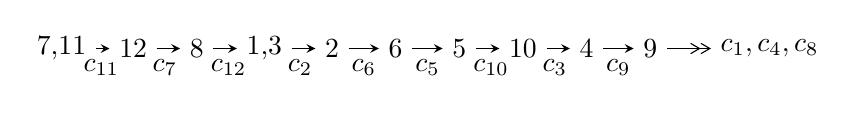
\begin{tikzpicture}[x=23pt, y=7pt]
	% node
	\node (A0) at (-1/8, 0) {7,11};
	\node (A1) at (1, 0) {12};
	\node (A2) at (2, 0) {8};
	\node (A3) at (49/16, 0) {1,3};
	\node (A4) at (33/8, 0) {2};
	\node (A5) at (41/8, 0) {6};
	\node (A6) at (49/8, 0) {5};
	\node (A7) at (57/8, 0) {10};
	\node (A8) at (65/8, 0) {4};
	\node (A9) at (73/8, 0) {9};
	\node (C1) at (1/2, -1) {$c_{11}$};
	\node (C2) at (3/2, -1) {$c_{7}$};
	\node (C3) at (5/2, -1) {$c_{12}$};
	\node (C4) at (29/8, -1) {$c_{2}$};
	\node (C5) at (37/8, -1) {$c_{6}$};
	\node (C6) at (45/8, -1) {$c_{5}$};
	\node (C7) at (53/8, -1) {$c_{10}$};
	\node (C8) at (61/8, -1) {$c_{3}$};
	\node (C9) at (69/8, -1) {$c_{9}$};
	\node (A10) at (11, 0) {$c_{1},c_{4},c_{8}$};

	% edge
	\draw[->,>=stealth]	
	(A0) edge (A1) (A1) edge (A2) (A2) edge (A3) (A3) edge (A4) (A4) edge (A5) (A5) edge (A6) (A6) edge (A7) (A7) edge (A8) (A8) edge (A9) ;
	\draw[->>,>={angle 60}]	
	(A9) edge (A10);
\end{tikzpicture} \\ 

\end{tabular} \\

\footnotetext{
The image of knot diagram is generated by the software ``\textbf{Draw programme}" developed by Andrew Bartholomew(\url{http://www.layer8.co.uk/maths/draw/index.htm\#Running-draw}), where we modified some parts for our purpose(\url{https://github.com/CATsTAILs/LinksPainter}).
}\phantom \\ \newline 
\centering \textbf{Ideals for irreducible components\footnotemark of $X_{\text{par}}$} 
 
\begin{align*}
I^u_{1}&=\langle 
9.69782\times10^{536} u^{139}-2.25657\times10^{536} u^{138}+\cdots+6.06990\times10^{539} b+5.03879\times10^{539},\\
\phantom{I^u_{1}}&\phantom{= \langle  }2.09110\times10^{539} u^{139}-1.68892\times10^{539} u^{138}+\cdots+5.15941\times10^{541} a-1.14839\times10^{541},\\
\phantom{I^u_{1}}&\phantom{= \langle  }u^{140}- u^{139}+\cdots+1003 u-289\rangle \\
I^u_{2}&=\langle 
-186986226 u^{33}+327109657 u^{32}+\cdots+86350699 b-1171458903,\\
\phantom{I^u_{2}}&\phantom{= \langle  }1805845965 u^{33}-920160738 u^{32}+\cdots+86350699 a+6335297871,\;u^{34}-22 u^{32}+\cdots+10 u+1\rangle \\
\\
\end{align*}
\raggedright * 2 irreducible components of $\dim_{\mathbb{C}}=0$, with total 174 representations.\\
\footnotetext{All coefficients of polynomials are rational numbers. But the coefficients are sometimes approximated in decimal forms when there is not enough margin.}
\newpage
\renewcommand{\arraystretch}{1}
\centering \section*{I. $I^u_{1}= \langle 9.70\times10^{536} u^{139}-2.26\times10^{536} u^{138}+\cdots+6.07\times10^{539} b+5.04\times10^{539},\;2.09\times10^{539} u^{139}-1.69\times10^{539} u^{138}+\cdots+5.16\times10^{541} a-1.15\times10^{541},\;u^{140}- u^{139}+\cdots+1003 u-289 \rangle$}
\flushleft \textbf{(i) Arc colorings}\\
\begin{tabular}{m{7pt} m{180pt} m{7pt} m{180pt} }
\flushright $a_{7}=$&$\begin{pmatrix}0\\u\end{pmatrix}$ \\
\flushright $a_{11}=$&$\begin{pmatrix}1\\0\end{pmatrix}$ \\
\flushright $a_{12}=$&$\begin{pmatrix}1\\u^2\end{pmatrix}$ \\
\flushright $a_{8}=$&$\begin{pmatrix}- u\\- u^3+u\end{pmatrix}$ \\
\flushright $a_{1}=$&$\begin{pmatrix}- u^2+1\\- u^4+2 u^2\end{pmatrix}$ \\
\flushright $a_{3}=$&$\begin{pmatrix}-0.00405297 u^{139}+0.00327347 u^{138}+\cdots+3.21409 u+0.222581\\-0.00159769 u^{139}+0.000371764 u^{138}+\cdots+2.12271 u-0.830128\end{pmatrix}$ \\
\flushright $a_{2}=$&$\begin{pmatrix}-0.00565066 u^{139}+0.00364523 u^{138}+\cdots+5.33680 u-0.607546\\-0.00159769 u^{139}+0.000371764 u^{138}+\cdots+2.12271 u-0.830128\end{pmatrix}$ \\
\flushright $a_{6}=$&$\begin{pmatrix}0.00200581 u^{139}+0.00496507 u^{138}+\cdots-6.08461 u+3.72627\\-0.000810012 u^{139}+0.000938180 u^{138}+\cdots+0.913658 u+0.556043\end{pmatrix}$ \\
\flushright $a_{5}=$&$\begin{pmatrix}0.00402005 u^{139}-0.00217381 u^{138}+\cdots-5.07444 u+0.659975\\0.000571152 u^{139}-0.00100493 u^{138}+\cdots-0.805524 u+0.766408\end{pmatrix}$ \\
\flushright $a_{10}=$&$\begin{pmatrix}0.00270227 u^{139}-0.00279415 u^{138}+\cdots-1.21625 u+4.64222\\-0.00228002 u^{139}+0.00212213 u^{138}+\cdots+3.56568 u-0.996732\end{pmatrix}$ \\
\flushright $a_{4}=$&$\begin{pmatrix}0.00489730 u^{139}-0.00549964 u^{138}+\cdots-8.88933 u+3.90747\\0.0000696783 u^{139}-0.00146228 u^{138}+\cdots+1.57653 u+0.256233\end{pmatrix}$ \\
\flushright $a_{9}=$&$\begin{pmatrix}0.00261727 u^{139}-0.00177802 u^{138}+\cdots-0.497087 u+4.05204\\-0.00181158 u^{139}+0.00219701 u^{138}+\cdots+2.86224 u-0.820622\end{pmatrix}$\\&\end{tabular}
\flushleft \textbf{(ii) Obstruction class $= -1$}\\~\\
\flushleft \textbf{(iii) Cusp Shapes $= -0.0120913 u^{139}+0.00925037 u^{138}+\cdots-5.95755 u-14.8088$}\\~\\
\newpage\renewcommand{\arraystretch}{1}
\flushleft \textbf{(iv) u-Polynomials at the component}\newline \\
\begin{tabular}{m{50pt}|m{274pt}}
Crossings & \hspace{64pt}u-Polynomials at each crossing \\
\hline $$\begin{aligned}c_{1}\end{aligned}$$&$\begin{aligned}
&u^{140}+4 u^{139}+\cdots-9 u+1
\end{aligned}$\\
\hline $$\begin{aligned}c_{2}\end{aligned}$$&$\begin{aligned}
&u^{140}-2 u^{139}+\cdots+333381 u-48473
\end{aligned}$\\
\hline $$\begin{aligned}c_{3}\end{aligned}$$&$\begin{aligned}
&u^{140}-2 u^{139}+\cdots-41435571198 u-5037373313
\end{aligned}$\\
\hline $$\begin{aligned}c_{4},c_{8}\end{aligned}$$&$\begin{aligned}
&u^{140}+41 u^{138}+\cdots-3278 u-326
\end{aligned}$\\
\hline $$\begin{aligned}c_{5}\end{aligned}$$&$\begin{aligned}
&u^{140}-36 u^{138}+\cdots+1736923383 u+361950067
\end{aligned}$\\
\hline $$\begin{aligned}c_{6}\end{aligned}$$&$\begin{aligned}
&u^{140}-8 u^{139}+\cdots+106962 u+10082
\end{aligned}$\\
\hline $$\begin{aligned}c_{7},c_{11},c_{12}\end{aligned}$$&$\begin{aligned}
&u^{140}- u^{139}+\cdots+1003 u-289
\end{aligned}$\\
\hline $$\begin{aligned}c_{9}\end{aligned}$$&$\begin{aligned}
&u^{140}- u^{139}+\cdots+31 u-211
\end{aligned}$\\
\hline $$\begin{aligned}c_{10}\end{aligned}$$&$\begin{aligned}
&u^{140}+3 u^{139}+\cdots+14 u-1
\end{aligned}$\\
\hline
\end{tabular}\\~\\
\newpage\renewcommand{\arraystretch}{1}
\flushleft \textbf{(v) Riley Polynomials at the component}\newline \\
\begin{tabular}{m{50pt}|m{274pt}}
Crossings & \hspace{64pt}Riley Polynomials at each crossing \\
\hline $$\begin{aligned}c_{1}\end{aligned}$$&$\begin{aligned}
&y^{140}+10 y^{139}+\cdots+27 y+1
\end{aligned}$\\
\hline $$\begin{aligned}c_{2}\end{aligned}$$&$\begin{aligned}
&y^{140}-40 y^{139}+\cdots-91720535629 y+2349631729
\end{aligned}$\\
\hline $$\begin{aligned}c_{3}\end{aligned}$$&$\begin{aligned}
&y^{140}+84 y^{139}+\cdots+9.52\times10^{20} y+2.54\times10^{19}
\end{aligned}$\\
\hline $$\begin{aligned}c_{4},c_{8}\end{aligned}$$&$\begin{aligned}
&y^{140}+82 y^{139}+\cdots+3039300 y+106276
\end{aligned}$\\
\hline $$\begin{aligned}c_{5}\end{aligned}$$&$\begin{aligned}
&y^{140}-72 y^{139}+\cdots-3.85\times10^{18} y+1.31\times10^{17}
\end{aligned}$\\
\hline $$\begin{aligned}c_{6}\end{aligned}$$&$\begin{aligned}
&y^{140}+50 y^{139}+\cdots-13461745852 y+101646724
\end{aligned}$\\
\hline $$\begin{aligned}c_{7},c_{11},c_{12}\end{aligned}$$&$\begin{aligned}
&y^{140}-159 y^{139}+\cdots-199121 y+83521
\end{aligned}$\\
\hline $$\begin{aligned}c_{9}\end{aligned}$$&$\begin{aligned}
&y^{140}-17 y^{139}+\cdots-3596401 y+44521
\end{aligned}$\\
\hline $$\begin{aligned}c_{10}\end{aligned}$$&$\begin{aligned}
&y^{140}+11 y^{139}+\cdots+18 y+1
\end{aligned}$\\
\hline
\end{tabular}\\~\\
\newpage\flushleft \textbf{(vi) Complex Volumes and Cusp Shapes}
$$\begin{array}{c|c|c}  
\text{Solutions to }I^u_{1}& \I (\text{vol} + \sqrt{-1}CS) & \text{Cusp shape}\\
 \hline 
\begin{aligned}
u &= -0.664700 + 0.764460 I \\
a &= \phantom{-}0.786549 - 0.391919 I \\
b &= -0.777311 - 0.272732 I\end{aligned}
 & -4.21163 + 0.44946 I & \phantom{-0.000000 } 0 \\ \hline\begin{aligned}
u &= -0.664700 - 0.764460 I \\
a &= \phantom{-}0.786549 + 0.391919 I \\
b &= -0.777311 + 0.272732 I\end{aligned}
 & -4.21163 - 0.44946 I & \phantom{-0.000000 } 0 \\ \hline\begin{aligned}
u &= \phantom{-}0.723613 + 0.663890 I \\
a &= \phantom{-}0.100235 + 1.407650 I \\
b &= -1.098430 - 0.770465 I\end{aligned}
 & -4.29384 - 9.41106 I & \phantom{-0.000000 } 0 \\ \hline\begin{aligned}
u &= \phantom{-}0.723613 - 0.663890 I \\
a &= \phantom{-}0.100235 - 1.407650 I \\
b &= -1.098430 + 0.770465 I\end{aligned}
 & -4.29384 + 9.41106 I & \phantom{-0.000000 } 0 \\ \hline\begin{aligned}
u &= -0.875504 + 0.391347 I \\
a &= -0.694523 + 0.387506 I \\
b &= \phantom{-}0.785277 + 0.019643 I\end{aligned}
 & -1.105740 - 0.505263 I & \phantom{-0.000000 } 0 \\ \hline\begin{aligned}
u &= -0.875504 - 0.391347 I \\
a &= -0.694523 - 0.387506 I \\
b &= \phantom{-}0.785277 - 0.019643 I\end{aligned}
 & -1.105740 + 0.505263 I & \phantom{-0.000000 } 0 \\ \hline\begin{aligned}
u &= -0.733482 + 0.494442 I \\
a &= \phantom{-}1.337570 - 0.211604 I \\
b &= -0.097656 - 0.212794 I\end{aligned}
 & \phantom{-}1.98403 - 3.21396 I & \phantom{-0.000000 } 0 \\ \hline\begin{aligned}
u &= -0.733482 - 0.494442 I \\
a &= \phantom{-}1.337570 + 0.211604 I \\
b &= -0.097656 + 0.212794 I\end{aligned}
 & \phantom{-}1.98403 + 3.21396 I & \phantom{-0.000000 } 0 \\ \hline\begin{aligned}
u &= \phantom{-}1.061780 + 0.419066 I \\
a &= -0.466473 - 0.043502 I \\
b &= \phantom{-}0.186946 - 0.630288 I\end{aligned}
 & \phantom{-}2.41235 - 5.18322 I & \phantom{-0.000000 } 0 \\ \hline\begin{aligned}
u &= \phantom{-}1.061780 - 0.419066 I \\
a &= -0.466473 + 0.043502 I \\
b &= \phantom{-}0.186946 + 0.630288 I\end{aligned}
 & \phantom{-}2.41235 + 5.18322 I & \phantom{-0.000000 } 0\\
 \hline 
 \end{array}$$\newpage$$\begin{array}{c|c|c}  
\text{Solutions to }I^u_{1}& \I (\text{vol} + \sqrt{-1}CS) & \text{Cusp shape}\\
 \hline 
\begin{aligned}
u &= -0.842849 + 0.091369 I \\
a &= -0.389431 - 0.059980 I \\
b &= \phantom{-}0.589549 + 0.329056 I\end{aligned}
 & -0.971976 + 0.163551 I & \phantom{-0.000000 } 0 \\ \hline\begin{aligned}
u &= -0.842849 - 0.091369 I \\
a &= -0.389431 + 0.059980 I \\
b &= \phantom{-}0.589549 - 0.329056 I\end{aligned}
 & -0.971976 - 0.163551 I & \phantom{-0.000000 } 0 \\ \hline\begin{aligned}
u &= \phantom{-}0.797009 + 0.237221 I \\
a &= \phantom{-}0.61591 - 1.60801 I \\
b &= \phantom{-}0.841277 + 0.591255 I\end{aligned}
 & -1.00052 - 4.05079 I & \phantom{-0.000000 } 0 \\ \hline\begin{aligned}
u &= \phantom{-}0.797009 - 0.237221 I \\
a &= \phantom{-}0.61591 + 1.60801 I \\
b &= \phantom{-}0.841277 - 0.591255 I\end{aligned}
 & -1.00052 + 4.05079 I & \phantom{-0.000000 } 0 \\ \hline\begin{aligned}
u &= -0.695414 + 0.416816 I \\
a &= \phantom{-}0.415690 - 1.231430 I \\
b &= \phantom{-}0.747231 + 1.026780 I\end{aligned}
 & -0.84448 - 4.06575 I & \phantom{-0.000000 } 0 \\ \hline\begin{aligned}
u &= -0.695414 - 0.416816 I \\
a &= \phantom{-}0.415690 + 1.231430 I \\
b &= \phantom{-}0.747231 - 1.026780 I\end{aligned}
 & -0.84448 + 4.06575 I & \phantom{-0.000000 } 0 \\ \hline\begin{aligned}
u &= -0.784025 + 0.909426 I \\
a &= \phantom{-}0.199354 - 1.141200 I \\
b &= -1.039980 + 0.900244 I\end{aligned}
 & -0.7502 + 14.8929 I & \phantom{-0.000000 } 0 \\ \hline\begin{aligned}
u &= -0.784025 - 0.909426 I \\
a &= \phantom{-}0.199354 + 1.141200 I \\
b &= -1.039980 - 0.900244 I\end{aligned}
 & -0.7502 - 14.8929 I & \phantom{-0.000000 } 0 \\ \hline\begin{aligned}
u &= -0.427709 + 1.129230 I \\
a &= -0.486121 + 0.803738 I \\
b &= \phantom{-}0.917993 - 0.745761 I\end{aligned}
 & -2.94428 + 5.11499 I & \phantom{-0.000000 } 0 \\ \hline\begin{aligned}
u &= -0.427709 - 1.129230 I \\
a &= -0.486121 - 0.803738 I \\
b &= \phantom{-}0.917993 + 0.745761 I\end{aligned}
 & -2.94428 - 5.11499 I & \phantom{-0.000000 } 0\\
 \hline 
 \end{array}$$\newpage$$\begin{array}{c|c|c}  
\text{Solutions to }I^u_{1}& \I (\text{vol} + \sqrt{-1}CS) & \text{Cusp shape}\\
 \hline 
\begin{aligned}
u &= \phantom{-}0.110880 + 0.770452 I \\
a &= -1.176030 + 0.513815 I \\
b &= \phantom{-}0.959095 - 0.550578 I\end{aligned}
 & -2.67355 + 4.62927 I & \phantom{-0.000000 } 0 \\ \hline\begin{aligned}
u &= \phantom{-}0.110880 - 0.770452 I \\
a &= -1.176030 - 0.513815 I \\
b &= \phantom{-}0.959095 + 0.550578 I\end{aligned}
 & -2.67355 - 4.62927 I & \phantom{-0.000000 } 0 \\ \hline\begin{aligned}
u &= \phantom{-}0.579144 + 0.513632 I \\
a &= -0.502537 - 0.140677 I \\
b &= \phantom{-}0.652717 - 0.875480 I\end{aligned}
 & \phantom{-}3.12611 + 4.01064 I & \phantom{-0.000000 } 0 \\ \hline\begin{aligned}
u &= \phantom{-}0.579144 - 0.513632 I \\
a &= -0.502537 + 0.140677 I \\
b &= \phantom{-}0.652717 + 0.875480 I\end{aligned}
 & \phantom{-}3.12611 - 4.01064 I & \phantom{-0.000000 } 0 \\ \hline\begin{aligned}
u &= \phantom{-}0.662666 + 0.391153 I \\
a &= -0.14133 - 1.72463 I \\
b &= \phantom{-}0.994817 + 0.972515 I\end{aligned}
 & -1.03835 - 6.46385 I & \phantom{-0.000000 } 0 \\ \hline\begin{aligned}
u &= \phantom{-}0.662666 - 0.391153 I \\
a &= -0.14133 + 1.72463 I \\
b &= \phantom{-}0.994817 - 0.972515 I\end{aligned}
 & -1.03835 + 6.46385 I & \phantom{-0.000000 } 0 \\ \hline\begin{aligned}
u &= \phantom{-}0.703698 + 0.296351 I \\
a &= \phantom{-}1.69296 + 0.67637 I \\
b &= \phantom{-}1.023900 - 0.024241 I\end{aligned}
 & -1.23542 + 4.69462 I & \phantom{-0.000000 } 0 \\ \hline\begin{aligned}
u &= \phantom{-}0.703698 - 0.296351 I \\
a &= \phantom{-}1.69296 - 0.67637 I \\
b &= \phantom{-}1.023900 + 0.024241 I\end{aligned}
 & -1.23542 - 4.69462 I & \phantom{-0.000000 } 0 \\ \hline\begin{aligned}
u &= -1.169030 + 0.406222 I \\
a &= \phantom{-}0.374439 + 0.919876 I \\
b &= \phantom{-}1.01034 - 0.99123 I\end{aligned}
 & \phantom{-}1.69637 + 3.05376 I & \phantom{-0.000000 } 0 \\ \hline\begin{aligned}
u &= -1.169030 - 0.406222 I \\
a &= \phantom{-}0.374439 - 0.919876 I \\
b &= \phantom{-}1.01034 + 0.99123 I\end{aligned}
 & \phantom{-}1.69637 - 3.05376 I & \phantom{-0.000000 } 0\\
 \hline 
 \end{array}$$\newpage$$\begin{array}{c|c|c}  
\text{Solutions to }I^u_{1}& \I (\text{vol} + \sqrt{-1}CS) & \text{Cusp shape}\\
 \hline 
\begin{aligned}
u &= \phantom{-}0.055131 + 0.760060 I \\
a &= \phantom{-}0.654166 + 1.059530 I \\
b &= -0.564034 - 0.881275 I\end{aligned}
 & \phantom{-}5.41822 + 1.05469 I & \phantom{-0.000000 } 0 \\ \hline\begin{aligned}
u &= \phantom{-}0.055131 - 0.760060 I \\
a &= \phantom{-}0.654166 - 1.059530 I \\
b &= -0.564034 + 0.881275 I\end{aligned}
 & \phantom{-}5.41822 - 1.05469 I & \phantom{-0.000000 } 0 \\ \hline\begin{aligned}
u &= \phantom{-}0.512374 + 0.531816 I \\
a &= -0.124478 + 1.229360 I \\
b &= -1.19410 - 0.93878 I\end{aligned}
 & \phantom{-}3.24255 - 7.63630 I & \phantom{-0.000000 } 0 \\ \hline\begin{aligned}
u &= \phantom{-}0.512374 - 0.531816 I \\
a &= -0.124478 - 1.229360 I \\
b &= -1.19410 + 0.93878 I\end{aligned}
 & \phantom{-}3.24255 + 7.63630 I & \phantom{-0.000000 } 0 \\ \hline\begin{aligned}
u &= -0.668082 + 0.296672 I \\
a &= -0.319331 + 0.795469 I \\
b &= \phantom{-}0.962171 - 0.600319 I\end{aligned}
 & -1.87716 + 0.12463 I & \phantom{-0.000000 } 0 \\ \hline\begin{aligned}
u &= -0.668082 - 0.296672 I \\
a &= -0.319331 - 0.795469 I \\
b &= \phantom{-}0.962171 + 0.600319 I\end{aligned}
 & -1.87716 - 0.12463 I & \phantom{-0.000000 } 0 \\ \hline\begin{aligned}
u &= \phantom{-}0.574185 + 0.440435 I \\
a &= \phantom{-}0.971814 - 0.681398 I \\
b &= \phantom{-}0.036914 + 0.599146 I\end{aligned}
 & \phantom{-}2.57035 - 1.43023 I & \phantom{-0.000000 } 0 \\ \hline\begin{aligned}
u &= \phantom{-}0.574185 - 0.440435 I \\
a &= \phantom{-}0.971814 + 0.681398 I \\
b &= \phantom{-}0.036914 - 0.599146 I\end{aligned}
 & \phantom{-}2.57035 + 1.43023 I & \phantom{-0.000000 } 0 \\ \hline\begin{aligned}
u &= \phantom{-}0.462670 + 0.554740 I \\
a &= \phantom{-}0.28947 - 1.44217 I \\
b &= \phantom{-}0.268987 + 0.813665 I\end{aligned}
 & \phantom{-}2.90772 - 2.18120 I & \phantom{-0.000000 } 0 \\ \hline\begin{aligned}
u &= \phantom{-}0.462670 - 0.554740 I \\
a &= \phantom{-}0.28947 + 1.44217 I \\
b &= \phantom{-}0.268987 - 0.813665 I\end{aligned}
 & \phantom{-}2.90772 + 2.18120 I & \phantom{-0.000000 } 0\\
 \hline 
 \end{array}$$\newpage$$\begin{array}{c|c|c}  
\text{Solutions to }I^u_{1}& \I (\text{vol} + \sqrt{-1}CS) & \text{Cusp shape}\\
 \hline 
\begin{aligned}
u &= -0.325781 + 0.637531 I \\
a &= \phantom{-}0.73161 - 1.30044 I \\
b &= -0.646866 + 0.111992 I\end{aligned}
 & -0.28044 + 3.17028 I & \phantom{-0.000000 } 0 \\ \hline\begin{aligned}
u &= -0.325781 - 0.637531 I \\
a &= \phantom{-}0.73161 + 1.30044 I \\
b &= -0.646866 - 0.111992 I\end{aligned}
 & -0.28044 - 3.17028 I & \phantom{-0.000000 } 0 \\ \hline\begin{aligned}
u &= \phantom{-}0.633748 + 1.166710 I \\
a &= \phantom{-}0.586035 + 0.085599 I \\
b &= -0.750696 + 0.232676 I\end{aligned}
 & -0.87696 - 5.20914 I & \phantom{-0.000000 } 0 \\ \hline\begin{aligned}
u &= \phantom{-}0.633748 - 1.166710 I \\
a &= \phantom{-}0.586035 - 0.085599 I \\
b &= -0.750696 - 0.232676 I\end{aligned}
 & -0.87696 + 5.20914 I & \phantom{-0.000000 } 0 \\ \hline\begin{aligned}
u &= \phantom{-}0.915236 + 0.974210 I \\
a &= -0.129646 - 0.943460 I \\
b &= \phantom{-}0.966530 + 0.747208 I\end{aligned}
 & -1.83283 - 2.03560 I & \phantom{-0.000000 } 0 \\ \hline\begin{aligned}
u &= \phantom{-}0.915236 - 0.974210 I \\
a &= -0.129646 + 0.943460 I \\
b &= \phantom{-}0.966530 - 0.747208 I\end{aligned}
 & -1.83283 + 2.03560 I & \phantom{-0.000000 } 0 \\ \hline\begin{aligned}
u &= -0.397448 + 0.491112 I \\
a &= -2.64127 - 0.55813 I \\
b &= -0.472527 + 0.413037 I\end{aligned}
 & \phantom{-}0.04254 + 7.33492 I & -9.9382 - 14.3032 I \\ \hline\begin{aligned}
u &= -0.397448 - 0.491112 I \\
a &= -2.64127 + 0.55813 I \\
b &= -0.472527 - 0.413037 I\end{aligned}
 & \phantom{-}0.04254 - 7.33492 I & -9.9382 + 14.3032 I \\ \hline\begin{aligned}
u &= -0.459772 + 1.299100 I \\
a &= -0.634517 - 0.229659 I \\
b &= \phantom{-}0.684407 + 0.575593 I\end{aligned}
 & \phantom{-}0.44709 - 7.98394 I & \phantom{-0.000000 } 0 \\ \hline\begin{aligned}
u &= -0.459772 - 1.299100 I \\
a &= -0.634517 + 0.229659 I \\
b &= \phantom{-}0.684407 - 0.575593 I\end{aligned}
 & \phantom{-}0.44709 + 7.98394 I & \phantom{-0.000000 } 0\\
 \hline 
 \end{array}$$\newpage$$\begin{array}{c|c|c}  
\text{Solutions to }I^u_{1}& \I (\text{vol} + \sqrt{-1}CS) & \text{Cusp shape}\\
 \hline 
\begin{aligned}
u &= \phantom{-}0.439314 + 0.438525 I \\
a &= -0.260113 - 1.107590 I \\
b &= -1.19873 + 1.08257 I\end{aligned}
 & -0.48464 - 7.47319 I & -11.6774 + 11.9215 I \\ \hline\begin{aligned}
u &= \phantom{-}0.439314 - 0.438525 I \\
a &= -0.260113 + 1.107590 I \\
b &= -1.19873 - 1.08257 I\end{aligned}
 & -0.48464 + 7.47319 I & -11.6774 - 11.9215 I \\ \hline\begin{aligned}
u &= -0.396768 + 0.443070 I \\
a &= -0.89644 + 2.45471 I \\
b &= \phantom{-}0.375721 - 0.782823 I\end{aligned}
 & \phantom{-}2.98407 + 6.46449 I & \phantom{-}0.34509 - 10.66849 I \\ \hline\begin{aligned}
u &= -0.396768 - 0.443070 I \\
a &= -0.89644 - 2.45471 I \\
b &= \phantom{-}0.375721 + 0.782823 I\end{aligned}
 & \phantom{-}2.98407 - 6.46449 I & \phantom{-}0.34509 + 10.66849 I \\ \hline\begin{aligned}
u &= -0.191276 + 0.560807 I \\
a &= \phantom{-}1.38693 - 1.88511 I \\
b &= -0.847157 + 0.495383 I\end{aligned}
 & \phantom{-}0.99488 + 4.11864 I & \phantom{-}6.68742 - 8.04172 I \\ \hline\begin{aligned}
u &= -0.191276 - 0.560807 I \\
a &= \phantom{-}1.38693 + 1.88511 I \\
b &= -0.847157 - 0.495383 I\end{aligned}
 & \phantom{-}0.99488 - 4.11864 I & \phantom{-}6.68742 + 8.04172 I \\ \hline\begin{aligned}
u &= -0.512094 + 0.288469 I \\
a &= \phantom{-}0.201018 + 0.891256 I \\
b &= -0.70226 - 1.39420 I\end{aligned}
 & -2.57763 + 2.49455 I & -13.1614 - 11.8667 I \\ \hline\begin{aligned}
u &= -0.512094 - 0.288469 I \\
a &= \phantom{-}0.201018 - 0.891256 I \\
b &= -0.70226 + 1.39420 I\end{aligned}
 & -2.57763 - 2.49455 I & -13.1614 + 11.8667 I \\ \hline\begin{aligned}
u &= \phantom{-}0.312147 + 0.473730 I \\
a &= -0.851897 - 0.627104 I \\
b &= \phantom{-}0.992979 + 0.845993 I\end{aligned}
 & -1.64722 - 2.64192 I & -6.75968 + 7.82828 I \\ \hline\begin{aligned}
u &= \phantom{-}0.312147 - 0.473730 I \\
a &= -0.851897 + 0.627104 I \\
b &= \phantom{-}0.992979 - 0.845993 I\end{aligned}
 & -1.64722 + 2.64192 I & -6.75968 - 7.82828 I\\
 \hline 
 \end{array}$$\newpage$$\begin{array}{c|c|c}  
\text{Solutions to }I^u_{1}& \I (\text{vol} + \sqrt{-1}CS) & \text{Cusp shape}\\
 \hline 
\begin{aligned}
u &= -0.564449\phantom{ +0.000000I} \\
a &= \phantom{-}0.133288\phantom{ +0.000000I} \\
b &= \phantom{-}0.672795\phantom{ +0.000000I}\end{aligned}
 & -0.962744\phantom{ +0.000000I} & -10.1490\phantom{ +0.000000I} \\ \hline\begin{aligned}
u &= -1.43044 + 0.15138 I \\
a &= -0.115764 + 0.526391 I \\
b &= \phantom{-}0.782330 - 0.869276 I\end{aligned}
 & -3.57102 - 0.35621 I & \phantom{-0.000000 } 0 \\ \hline\begin{aligned}
u &= -1.43044 - 0.15138 I \\
a &= -0.115764 - 0.526391 I \\
b &= \phantom{-}0.782330 + 0.869276 I\end{aligned}
 & -3.57102 + 0.35621 I & \phantom{-0.000000 } 0 \\ \hline\begin{aligned}
u &= \phantom{-}1.45865 + 0.11674 I \\
a &= \phantom{-}0.64936 - 1.26547 I \\
b &= \phantom{-}1.006320 + 0.697960 I\end{aligned}
 & -4.44443 - 6.18107 I & \phantom{-0.000000 } 0 \\ \hline\begin{aligned}
u &= \phantom{-}1.45865 - 0.11674 I \\
a &= \phantom{-}0.64936 + 1.26547 I \\
b &= \phantom{-}1.006320 - 0.697960 I\end{aligned}
 & -4.44443 + 6.18107 I & \phantom{-0.000000 } 0 \\ \hline\begin{aligned}
u &= \phantom{-}1.46459 + 0.13353 I \\
a &= -1.213010 - 0.673295 I \\
b &= -0.792738 + 0.117029 I\end{aligned}
 & -7.91264 - 1.67664 I & \phantom{-0.000000 } 0 \\ \hline\begin{aligned}
u &= \phantom{-}1.46459 - 0.13353 I \\
a &= -1.213010 + 0.673295 I \\
b &= -0.792738 - 0.117029 I\end{aligned}
 & -7.91264 + 1.67664 I & \phantom{-0.000000 } 0 \\ \hline\begin{aligned}
u &= -1.47219 + 0.12110 I \\
a &= -0.231901 + 0.522863 I \\
b &= -1.54570 - 1.57835 I\end{aligned}
 & -8.19313 + 0.75936 I & \phantom{-0.000000 } 0 \\ \hline\begin{aligned}
u &= -1.47219 - 0.12110 I \\
a &= -0.231901 - 0.522863 I \\
b &= -1.54570 + 1.57835 I\end{aligned}
 & -8.19313 - 0.75936 I & \phantom{-0.000000 } 0 \\ \hline\begin{aligned}
u &= -1.48733 + 0.03501 I \\
a &= \phantom{-}0.322703 + 0.980063 I \\
b &= \phantom{-}0.724917 - 0.201965 I\end{aligned}
 & -5.89372 - 3.44747 I & \phantom{-0.000000 } 0\\
 \hline 
 \end{array}$$\newpage$$\begin{array}{c|c|c}  
\text{Solutions to }I^u_{1}& \I (\text{vol} + \sqrt{-1}CS) & \text{Cusp shape}\\
 \hline 
\begin{aligned}
u &= -1.48733 - 0.03501 I \\
a &= \phantom{-}0.322703 - 0.980063 I \\
b &= \phantom{-}0.724917 + 0.201965 I\end{aligned}
 & -5.89372 + 3.44747 I & \phantom{-0.000000 } 0 \\ \hline\begin{aligned}
u &= \phantom{-}1.48781 + 0.05381 I \\
a &= \phantom{-}0.752448 - 0.618143 I \\
b &= \phantom{-}1.59477 + 0.64458 I\end{aligned}
 & -4.93916 - 2.78367 I & \phantom{-0.000000 } 0 \\ \hline\begin{aligned}
u &= \phantom{-}1.48781 - 0.05381 I \\
a &= \phantom{-}0.752448 + 0.618143 I \\
b &= \phantom{-}1.59477 - 0.64458 I\end{aligned}
 & -4.93916 + 2.78367 I & \phantom{-0.000000 } 0 \\ \hline\begin{aligned}
u &= \phantom{-}0.503828 + 0.073523 I \\
a &= -2.44089 - 2.01714 I \\
b &= -0.545407 - 0.128755 I\end{aligned}
 & -3.64336 - 1.92912 I & -22.2195 + 4.5913 I \\ \hline\begin{aligned}
u &= \phantom{-}0.503828 - 0.073523 I \\
a &= -2.44089 + 2.01714 I \\
b &= -0.545407 + 0.128755 I\end{aligned}
 & -3.64336 + 1.92912 I & -22.2195 - 4.5913 I \\ \hline\begin{aligned}
u &= -1.48908 + 0.12089 I \\
a &= -0.060076 - 0.562281 I \\
b &= -1.302230 + 0.127007 I\end{aligned}
 & -8.02860 - 2.49175 I & \phantom{-0.000000 } 0 \\ \hline\begin{aligned}
u &= -1.48908 - 0.12089 I \\
a &= -0.060076 + 0.562281 I \\
b &= -1.302230 - 0.127007 I\end{aligned}
 & -8.02860 + 2.49175 I & \phantom{-0.000000 } 0 \\ \hline\begin{aligned}
u &= \phantom{-}1.47894 + 0.21321 I \\
a &= -0.658120 + 0.409281 I \\
b &= -0.755694 + 0.115306 I\end{aligned}
 & -5.65381 - 0.48158 I & \phantom{-0.000000 } 0 \\ \hline\begin{aligned}
u &= \phantom{-}1.47894 - 0.21321 I \\
a &= -0.658120 - 0.409281 I \\
b &= -0.755694 - 0.115306 I\end{aligned}
 & -5.65381 + 0.48158 I & \phantom{-0.000000 } 0 \\ \hline\begin{aligned}
u &= \phantom{-}1.49203 + 0.08952 I \\
a &= -0.427255 + 0.881362 I \\
b &= -1.48446 - 1.13266 I\end{aligned}
 & -8.45812 - 5.96609 I & \phantom{-0.000000 } 0\\
 \hline 
 \end{array}$$\newpage$$\begin{array}{c|c|c}  
\text{Solutions to }I^u_{1}& \I (\text{vol} + \sqrt{-1}CS) & \text{Cusp shape}\\
 \hline 
\begin{aligned}
u &= \phantom{-}1.49203 - 0.08952 I \\
a &= -0.427255 - 0.881362 I \\
b &= -1.48446 + 1.13266 I\end{aligned}
 & -8.45812 + 5.96609 I & \phantom{-0.000000 } 0 \\ \hline\begin{aligned}
u &= \phantom{-}1.48826 + 0.17864 I \\
a &= \phantom{-}0.535093 - 1.113330 I \\
b &= \phantom{-}0.823116 + 0.394357 I\end{aligned}
 & -6.31084 - 5.99967 I & \phantom{-0.000000 } 0 \\ \hline\begin{aligned}
u &= \phantom{-}1.48826 - 0.17864 I \\
a &= \phantom{-}0.535093 + 1.113330 I \\
b &= \phantom{-}0.823116 - 0.394357 I\end{aligned}
 & -6.31084 + 5.99967 I & \phantom{-0.000000 } 0 \\ \hline\begin{aligned}
u &= -0.335044 + 0.367577 I \\
a &= \phantom{-}2.03708 + 0.63434 I \\
b &= \phantom{-}0.726011 - 0.525189 I\end{aligned}
 & -2.09120 - 0.13055 I & -11.23045 - 3.27237 I \\ \hline\begin{aligned}
u &= -0.335044 - 0.367577 I \\
a &= \phantom{-}2.03708 - 0.63434 I \\
b &= \phantom{-}0.726011 + 0.525189 I\end{aligned}
 & -2.09120 + 0.13055 I & -11.23045 + 3.27237 I \\ \hline\begin{aligned}
u &= \phantom{-}1.50933 + 0.13545 I \\
a &= \phantom{-}1.61865 + 0.68437 I \\
b &= \phantom{-}0.541875 - 0.007146 I\end{aligned}
 & -6.33975 - 9.50478 I & \phantom{-0.000000 } 0 \\ \hline\begin{aligned}
u &= \phantom{-}1.50933 - 0.13545 I \\
a &= \phantom{-}1.61865 - 0.68437 I \\
b &= \phantom{-}0.541875 + 0.007146 I\end{aligned}
 & -6.33975 + 9.50478 I & \phantom{-0.000000 } 0 \\ \hline\begin{aligned}
u &= -1.51497 + 0.13006 I \\
a &= -0.185483 - 0.538002 I \\
b &= -1.68824 + 1.32651 I\end{aligned}
 & -7.94331 + 4.70663 I & \phantom{-0.000000 } 0 \\ \hline\begin{aligned}
u &= -1.51497 - 0.13006 I \\
a &= -0.185483 + 0.538002 I \\
b &= -1.68824 - 1.32651 I\end{aligned}
 & -7.94331 - 4.70663 I & \phantom{-0.000000 } 0 \\ \hline\begin{aligned}
u &= \phantom{-}1.52067 + 0.11940 I \\
a &= -0.289867 + 1.292590 I \\
b &= -0.475269 - 1.136580 I\end{aligned}
 & -3.51038 - 8.39205 I & \phantom{-0.000000 } 0\\
 \hline 
 \end{array}$$\newpage$$\begin{array}{c|c|c}  
\text{Solutions to }I^u_{1}& \I (\text{vol} + \sqrt{-1}CS) & \text{Cusp shape}\\
 \hline 
\begin{aligned}
u &= \phantom{-}1.52067 - 0.11940 I \\
a &= -0.289867 - 1.292590 I \\
b &= -0.475269 + 1.136580 I\end{aligned}
 & -3.51038 + 8.39205 I & \phantom{-0.000000 } 0 \\ \hline\begin{aligned}
u &= -1.51859 + 0.15663 I \\
a &= -0.527020 - 0.806732 I \\
b &= -0.554889 + 0.927513 I\end{aligned}
 & -3.66738 + 4.69280 I & \phantom{-0.000000 } 0 \\ \hline\begin{aligned}
u &= -1.51859 - 0.15663 I \\
a &= -0.527020 + 0.806732 I \\
b &= -0.554889 - 0.927513 I\end{aligned}
 & -3.66738 - 4.69280 I & \phantom{-0.000000 } 0 \\ \hline\begin{aligned}
u &= \phantom{-}1.52841\phantom{ +0.000000I} \\
a &= -0.713515\phantom{ +0.000000I} \\
b &= -1.27813\phantom{ +0.000000I}\end{aligned}
 & -7.81776\phantom{ +0.000000I} & \phantom{-0.000000 } 0 \\ \hline\begin{aligned}
u &= -1.53279 + 0.01394 I \\
a &= \phantom{-}1.14809 - 1.21363 I \\
b &= \phantom{-}0.620121 + 0.251284 I\end{aligned}
 & -10.52960 + 2.20106 I & \phantom{-0.000000 } 0 \\ \hline\begin{aligned}
u &= -1.53279 - 0.01394 I \\
a &= \phantom{-}1.14809 + 1.21363 I \\
b &= \phantom{-}0.620121 - 0.251284 I\end{aligned}
 & -10.52960 - 2.20106 I & \phantom{-0.000000 } 0 \\ \hline\begin{aligned}
u &= -1.52839 + 0.12828 I \\
a &= \phantom{-}0.081023 - 0.416786 I \\
b &= \phantom{-}1.48690 + 1.88540 I\end{aligned}
 & -7.13324 + 9.48597 I & \phantom{-0.000000 } 0 \\ \hline\begin{aligned}
u &= -1.52839 - 0.12828 I \\
a &= \phantom{-}0.081023 + 0.416786 I \\
b &= \phantom{-}1.48690 - 1.88540 I\end{aligned}
 & -7.13324 - 9.48597 I & \phantom{-0.000000 } 0 \\ \hline\begin{aligned}
u &= \phantom{-}1.54665 + 0.05449 I \\
a &= \phantom{-}0.009875 + 0.380881 I \\
b &= \phantom{-}0.95023 - 2.11525 I\end{aligned}
 & -9.57912 - 3.58725 I & \phantom{-0.000000 } 0 \\ \hline\begin{aligned}
u &= \phantom{-}1.54665 - 0.05449 I \\
a &= \phantom{-}0.009875 - 0.380881 I \\
b &= \phantom{-}0.95023 + 2.11525 I\end{aligned}
 & -9.57912 + 3.58725 I & \phantom{-0.000000 } 0\\
 \hline 
 \end{array}$$\newpage$$\begin{array}{c|c|c}  
\text{Solutions to }I^u_{1}& \I (\text{vol} + \sqrt{-1}CS) & \text{Cusp shape}\\
 \hline 
\begin{aligned}
u &= -1.54101 + 0.15944 I \\
a &= \phantom{-}0.564425 + 0.524302 I \\
b &= \phantom{-}1.75708 - 0.92401 I\end{aligned}
 & -3.63309 + 10.12680 I & \phantom{-0.000000 } 0 \\ \hline\begin{aligned}
u &= -1.54101 - 0.15944 I \\
a &= \phantom{-}0.564425 - 0.524302 I \\
b &= \phantom{-}1.75708 + 0.92401 I\end{aligned}
 & -3.63309 - 10.12680 I & \phantom{-0.000000 } 0 \\ \hline\begin{aligned}
u &= -1.56856 + 0.00769 I \\
a &= -0.87398 + 1.15965 I \\
b &= -0.719647 - 0.558022 I\end{aligned}
 & -9.07794 - 4.17420 I & \phantom{-0.000000 } 0 \\ \hline\begin{aligned}
u &= -1.56856 - 0.00769 I \\
a &= -0.87398 - 1.15965 I \\
b &= -0.719647 + 0.558022 I\end{aligned}
 & -9.07794 + 4.17420 I & \phantom{-0.000000 } 0 \\ \hline\begin{aligned}
u &= -1.57737 + 0.02561 I \\
a &= -0.621805 - 0.176074 I \\
b &= -0.638593 - 0.178351 I\end{aligned}
 & -5.01387 - 2.33379 I & \phantom{-0.000000 } 0 \\ \hline\begin{aligned}
u &= -1.57737 - 0.02561 I \\
a &= -0.621805 + 0.176074 I \\
b &= -0.638593 + 0.178351 I\end{aligned}
 & -5.01387 + 2.33379 I & \phantom{-0.000000 } 0 \\ \hline\begin{aligned}
u &= -0.108930 + 0.404335 I \\
a &= -1.95782 + 1.65702 I \\
b &= \phantom{-}1.168180 - 0.645412 I\end{aligned}
 & -2.66601 + 4.44912 I & -15.4555 - 3.5906 I \\ \hline\begin{aligned}
u &= -0.108930 - 0.404335 I \\
a &= -1.95782 - 1.65702 I \\
b &= \phantom{-}1.168180 + 0.645412 I\end{aligned}
 & -2.66601 - 4.44912 I & -15.4555 + 3.5906 I \\ \hline\begin{aligned}
u &= \phantom{-}1.59026 + 0.06498 I \\
a &= -0.177485 + 0.499893 I \\
b &= -1.46257 - 1.12144 I\end{aligned}
 & -9.55332 - 1.37380 I & \phantom{-0.000000 } 0 \\ \hline\begin{aligned}
u &= \phantom{-}1.59026 - 0.06498 I \\
a &= -0.177485 - 0.499893 I \\
b &= -1.46257 + 1.12144 I\end{aligned}
 & -9.55332 + 1.37380 I & \phantom{-0.000000 } 0\\
 \hline 
 \end{array}$$\newpage$$\begin{array}{c|c|c}  
\text{Solutions to }I^u_{1}& \I (\text{vol} + \sqrt{-1}CS) & \text{Cusp shape}\\
 \hline 
\begin{aligned}
u &= -1.59423 + 0.11837 I \\
a &= -0.352989 - 0.889997 I \\
b &= -1.32213 + 1.32352 I\end{aligned}
 & -8.72906 + 8.38051 I & \phantom{-0.000000 } 0 \\ \hline\begin{aligned}
u &= -1.59423 - 0.11837 I \\
a &= -0.352989 + 0.889997 I \\
b &= -1.32213 - 1.32352 I\end{aligned}
 & -8.72906 - 8.38051 I & \phantom{-0.000000 } 0 \\ \hline\begin{aligned}
u &= -1.60372 + 0.21478 I \\
a &= \phantom{-}0.513235 + 0.943608 I \\
b &= \phantom{-}1.32832 - 0.91986 I\end{aligned}
 & -12.0451 + 12.7341 I & \phantom{-0.000000 } 0 \\ \hline\begin{aligned}
u &= -1.60372 - 0.21478 I \\
a &= \phantom{-}0.513235 - 0.943608 I \\
b &= \phantom{-}1.32832 + 0.91986 I\end{aligned}
 & -12.0451 - 12.7341 I & \phantom{-0.000000 } 0 \\ \hline\begin{aligned}
u &= \phantom{-}1.61829 + 0.08905 I \\
a &= -0.115496 + 0.480212 I \\
b &= -1.201190 - 0.645880 I\end{aligned}
 & -9.46916 - 1.00537 I & \phantom{-0.000000 } 0 \\ \hline\begin{aligned}
u &= \phantom{-}1.61829 - 0.08905 I \\
a &= -0.115496 - 0.480212 I \\
b &= -1.201190 + 0.645880 I\end{aligned}
 & -9.46916 + 1.00537 I & \phantom{-0.000000 } 0 \\ \hline\begin{aligned}
u &= \phantom{-}1.62968 + 0.05452 I \\
a &= -0.230254 - 0.511771 I \\
b &= -1.31338 + 1.55457 I\end{aligned}
 & -9.05093 + 2.51533 I & \phantom{-0.000000 } 0 \\ \hline\begin{aligned}
u &= \phantom{-}1.62968 - 0.05452 I \\
a &= -0.230254 + 0.511771 I \\
b &= -1.31338 - 1.55457 I\end{aligned}
 & -9.05093 - 2.51533 I & \phantom{-0.000000 } 0 \\ \hline\begin{aligned}
u &= \phantom{-}1.61209 + 0.25281 I \\
a &= \phantom{-}0.008322 - 0.664491 I \\
b &= \phantom{-}0.931965 + 0.237653 I\end{aligned}
 & -11.78290 - 4.33530 I & \phantom{-0.000000 } 0 \\ \hline\begin{aligned}
u &= \phantom{-}1.61209 - 0.25281 I \\
a &= \phantom{-}0.008322 + 0.664491 I \\
b &= \phantom{-}0.931965 - 0.237653 I\end{aligned}
 & -11.78290 + 4.33530 I & \phantom{-0.000000 } 0\\
 \hline 
 \end{array}$$\newpage$$\begin{array}{c|c|c}  
\text{Solutions to }I^u_{1}& \I (\text{vol} + \sqrt{-1}CS) & \text{Cusp shape}\\
 \hline 
\begin{aligned}
u &= \phantom{-}0.300912 + 0.205547 I \\
a &= \phantom{-}2.41558 + 2.51152 I \\
b &= -0.669129 + 0.407572 I\end{aligned}
 & \phantom{-}0.23225 + 4.08304 I & -16.4105 - 4.0590 I \\ \hline\begin{aligned}
u &= \phantom{-}0.300912 - 0.205547 I \\
a &= \phantom{-}2.41558 - 2.51152 I \\
b &= -0.669129 - 0.407572 I\end{aligned}
 & \phantom{-}0.23225 - 4.08304 I & -16.4105 + 4.0590 I \\ \hline\begin{aligned}
u &= \phantom{-}0.199111 + 0.298771 I \\
a &= \phantom{-}1.22881 + 1.87046 I \\
b &= \phantom{-}0.890082 - 0.895262 I\end{aligned}
 & -2.54694 + 0.86537 I & -12.46402 + 5.98089 I \\ \hline\begin{aligned}
u &= \phantom{-}0.199111 - 0.298771 I \\
a &= \phantom{-}1.22881 - 1.87046 I \\
b &= \phantom{-}0.890082 + 0.895262 I\end{aligned}
 & -2.54694 - 0.86537 I & -12.46402 - 5.98089 I \\ \hline\begin{aligned}
u &= \phantom{-}1.61375 + 0.36334 I \\
a &= -0.368619 + 0.873433 I \\
b &= -1.33880 - 0.95632 I\end{aligned}
 & -9.8237 - 10.4986 I & \phantom{-0.000000 } 0 \\ \hline\begin{aligned}
u &= \phantom{-}1.61375 - 0.36334 I \\
a &= -0.368619 - 0.873433 I \\
b &= -1.33880 + 0.95632 I\end{aligned}
 & -9.8237 + 10.4986 I & \phantom{-0.000000 } 0 \\ \hline\begin{aligned}
u &= \phantom{-}1.64173 + 0.29194 I \\
a &= \phantom{-}0.429051 - 0.914569 I \\
b &= \phantom{-}1.34940 + 1.02524 I\end{aligned}
 & -8.7098 - 19.4012 I & \phantom{-0.000000 } 0 \\ \hline\begin{aligned}
u &= \phantom{-}1.64173 - 0.29194 I \\
a &= \phantom{-}0.429051 + 0.914569 I \\
b &= \phantom{-}1.34940 - 1.02524 I\end{aligned}
 & -8.7098 + 19.4012 I & \phantom{-0.000000 } 0 \\ \hline\begin{aligned}
u &= -0.187115 + 0.267019 I \\
a &= \phantom{-}0.21996 - 3.10938 I \\
b &= -1.014640 + 0.389268 I\end{aligned}
 & \phantom{-}0.93632 + 1.85529 I & \phantom{-}1.08312 - 2.65422 I \\ \hline\begin{aligned}
u &= -0.187115 - 0.267019 I \\
a &= \phantom{-}0.21996 + 3.10938 I \\
b &= -1.014640 - 0.389268 I\end{aligned}
 & \phantom{-}0.93632 - 1.85529 I & \phantom{-}1.08312 + 2.65422 I\\
 \hline 
 \end{array}$$\newpage$$\begin{array}{c|c|c}  
\text{Solutions to }I^u_{1}& \I (\text{vol} + \sqrt{-1}CS) & \text{Cusp shape}\\
 \hline 
\begin{aligned}
u &= \phantom{-}0.076035 + 0.309971 I \\
a &= \phantom{-}2.55660 - 1.68509 I \\
b &= -0.708724 + 0.256940 I\end{aligned}
 & \phantom{-}1.01016 + 1.78617 I & -0.59593 - 2.45671 I \\ \hline\begin{aligned}
u &= \phantom{-}0.076035 - 0.309971 I \\
a &= \phantom{-}2.55660 + 1.68509 I \\
b &= -0.708724 - 0.256940 I\end{aligned}
 & \phantom{-}1.01016 - 1.78617 I & -0.59593 + 2.45671 I \\ \hline\begin{aligned}
u &= -1.67758 + 0.21213 I \\
a &= -0.447388 - 0.880625 I \\
b &= -1.23909 + 0.92102 I\end{aligned}
 & -10.76140 + 6.29072 I & \phantom{-0.000000 } 0 \\ \hline\begin{aligned}
u &= -1.67758 - 0.21213 I \\
a &= -0.447388 + 0.880625 I \\
b &= -1.23909 - 0.92102 I\end{aligned}
 & -10.76140 - 6.29072 I & \phantom{-0.000000 } 0 \\ \hline\begin{aligned}
u &= -1.66320 + 0.34428 I \\
a &= \phantom{-}0.002532 + 0.582245 I \\
b &= \phantom{-}1.022320 - 0.244740 I\end{aligned}
 & -8.53641 + 10.73160 I & \phantom{-0.000000 } 0 \\ \hline\begin{aligned}
u &= -1.66320 - 0.34428 I \\
a &= \phantom{-}0.002532 - 0.582245 I \\
b &= \phantom{-}1.022320 + 0.244740 I\end{aligned}
 & -8.53641 - 10.73160 I & \phantom{-0.000000 } 0 \\ \hline\begin{aligned}
u &= -1.82968 + 0.54136 I \\
a &= \phantom{-}0.063321 - 0.344650 I \\
b &= -0.723983 + 0.035174 I\end{aligned}
 & -7.56867 + 2.29891 I & \phantom{-0.000000 } 0 \\ \hline\begin{aligned}
u &= -1.82968 - 0.54136 I \\
a &= \phantom{-}0.063321 + 0.344650 I \\
b &= -0.723983 - 0.035174 I\end{aligned}
 & -7.56867 - 2.29891 I & \phantom{-0.000000 } 0 \\ \hline\begin{aligned}
u &= \phantom{-}2.04595 + 0.16785 I \\
a &= -0.053376 + 0.312098 I \\
b &= -0.511875 - 0.170646 I\end{aligned}
 & -8.05626 + 0.26551 I & \phantom{-0.000000 } 0 \\ \hline\begin{aligned}
u &= \phantom{-}2.04595 - 0.16785 I \\
a &= -0.053376 - 0.312098 I \\
b &= -0.511875 + 0.170646 I\end{aligned}
 & -8.05626 - 0.26551 I & \phantom{-0.000000 } 0\\
 \hline 
 \end{array}$$\newpage\newpage\renewcommand{\arraystretch}{1}
\centering \section*{II. $I^u_{2}= \langle -1.87\times10^{8} u^{33}+3.27\times10^{8} u^{32}+\cdots+8.64\times10^{7} b-1.17\times10^{9},\;1.81\times10^{9} u^{33}-9.20\times10^{8} u^{32}+\cdots+8.64\times10^{7} a+6.34\times10^{9},\;u^{34}-22 u^{32}+\cdots+10 u+1 \rangle$}
\flushleft \textbf{(i) Arc colorings}\\
\begin{tabular}{m{7pt} m{180pt} m{7pt} m{180pt} }
\flushright $a_{7}=$&$\begin{pmatrix}0\\u\end{pmatrix}$ \\
\flushright $a_{11}=$&$\begin{pmatrix}1\\0\end{pmatrix}$ \\
\flushright $a_{12}=$&$\begin{pmatrix}1\\u^2\end{pmatrix}$ \\
\flushright $a_{8}=$&$\begin{pmatrix}- u\\- u^3+u\end{pmatrix}$ \\
\flushright $a_{1}=$&$\begin{pmatrix}- u^2+1\\- u^4+2 u^2\end{pmatrix}$ \\
\flushright $a_{3}=$&$\begin{pmatrix}-20.9129 u^{33}+10.6561 u^{32}+\cdots-457.670 u-73.3671\\2.16543 u^{33}-3.78815 u^{32}+\cdots+81.8945 u+13.5663\end{pmatrix}$ \\
\flushright $a_{2}=$&$\begin{pmatrix}-18.7475 u^{33}+6.86794 u^{32}+\cdots-375.776 u-59.8008\\2.16543 u^{33}-3.78815 u^{32}+\cdots+81.8945 u+13.5663\end{pmatrix}$ \\
\flushright $a_{6}=$&$\begin{pmatrix}5.06829 u^{33}-6.67284 u^{32}+\cdots+17.1786 u-2.50160\\0.180126 u^{33}-3.86825 u^{32}+\cdots-97.1453 u-16.8136\end{pmatrix}$ \\
\flushright $a_{5}=$&$\begin{pmatrix}-8.79495 u^{33}+2.09806 u^{32}+\cdots-264.937 u-46.2246\\2.94152 u^{33}-5.16362 u^{32}+\cdots-51.1550 u-8.71002\end{pmatrix}$ \\
\flushright $a_{10}=$&$\begin{pmatrix}10.9766 u^{33}+2.51680 u^{32}+\cdots+310.285 u+52.7726\\-7.26168 u^{33}+9.08502 u^{32}+\cdots-79.8501 u-11.7365\end{pmatrix}$ \\
\flushright $a_{4}=$&$\begin{pmatrix}-16.9016 u^{33}+7.90644 u^{32}+\cdots-339.054 u-55.2055\\-0.163445 u^{33}-1.31578 u^{32}+\cdots+22.9550 u+4.29848\end{pmatrix}$ \\
\flushright $a_{9}=$&$\begin{pmatrix}0.910329 u^{33}+11.9905 u^{32}+\cdots+194.865 u+35.1480\\-9.87884 u^{33}+11.0194 u^{32}+\cdots-95.8747 u-14.1151\end{pmatrix}$\\&\end{tabular}
\flushleft \textbf{(ii) Obstruction class $= 1$}\\~\\
\flushleft \textbf{(iii) Cusp Shapes $= \frac{2794613904}{86350699} u^{33}-\frac{2574155598}{86350699} u^{32}+\cdots+\frac{37461769996}{86350699} u+\frac{4272649106}{86350699}$}\\~\\
\newpage\renewcommand{\arraystretch}{1}
\flushleft \textbf{(iv) u-Polynomials at the component}\newline \\
\begin{tabular}{m{50pt}|m{274pt}}
Crossings & \hspace{64pt}u-Polynomials at each crossing \\
\hline $$\begin{aligned}c_{1}\end{aligned}$$&$\begin{aligned}
&u^{34}-11 u^{33}+\cdots-2 u+1
\end{aligned}$\\
\hline $$\begin{aligned}c_{2}\end{aligned}$$&$\begin{aligned}
&u^{34}-3 u^{33}+\cdots-8 u+1
\end{aligned}$\\
\hline $$\begin{aligned}c_{3}\end{aligned}$$&$\begin{aligned}
&u^{34}- u^{33}+\cdots+7 u+1
\end{aligned}$\\
\hline $$\begin{aligned}c_{4}\end{aligned}$$&$\begin{aligned}
&u^{34}+u^{33}+\cdots+21 u^2+2
\end{aligned}$\\
\hline $$\begin{aligned}c_{5}\end{aligned}$$&$\begin{aligned}
&u^{34}-3 u^{33}+\cdots+18 u+1
\end{aligned}$\\
\hline $$\begin{aligned}c_{6}\end{aligned}$$&$\begin{aligned}
&u^{34}-3 u^{33}+\cdots-4 u+2
\end{aligned}$\\
\hline $$\begin{aligned}c_{7}\end{aligned}$$&$\begin{aligned}
&u^{34}-22 u^{32}+\cdots-10 u+1
\end{aligned}$\\
\hline $$\begin{aligned}c_{8}\end{aligned}$$&$\begin{aligned}
&u^{34}- u^{33}+\cdots+21 u^2+2
\end{aligned}$\\
\hline $$\begin{aligned}c_{9}\end{aligned}$$&$\begin{aligned}
&u^{34}+2 u^{33}+\cdots+4 u+1
\end{aligned}$\\
\hline $$\begin{aligned}c_{10}\end{aligned}$$&$\begin{aligned}
&u^{34}- u^{32}+\cdots+u+1
\end{aligned}$\\
\hline $$\begin{aligned}c_{11},c_{12}\end{aligned}$$&$\begin{aligned}
&u^{34}-22 u^{32}+\cdots+10 u+1
\end{aligned}$\\
\hline
\end{tabular}\\~\\
\newpage\renewcommand{\arraystretch}{1}
\flushleft \textbf{(v) Riley Polynomials at the component}\newline \\
\begin{tabular}{m{50pt}|m{274pt}}
Crossings & \hspace{64pt}Riley Polynomials at each crossing \\
\hline $$\begin{aligned}c_{1}\end{aligned}$$&$\begin{aligned}
&y^{34}+5 y^{33}+\cdots+6 y+1
\end{aligned}$\\
\hline $$\begin{aligned}c_{2}\end{aligned}$$&$\begin{aligned}
&y^{34}-9 y^{33}+\cdots-10 y+1
\end{aligned}$\\
\hline $$\begin{aligned}c_{3}\end{aligned}$$&$\begin{aligned}
&y^{34}+23 y^{33}+\cdots+31 y+1
\end{aligned}$\\
\hline $$\begin{aligned}c_{4},c_{8}\end{aligned}$$&$\begin{aligned}
&y^{34}+25 y^{33}+\cdots+84 y+4
\end{aligned}$\\
\hline $$\begin{aligned}c_{5}\end{aligned}$$&$\begin{aligned}
&y^{34}-17 y^{33}+\cdots-26 y+1
\end{aligned}$\\
\hline $$\begin{aligned}c_{6}\end{aligned}$$&$\begin{aligned}
&y^{34}+17 y^{33}+\cdots+44 y+4
\end{aligned}$\\
\hline $$\begin{aligned}c_{7},c_{11},c_{12}\end{aligned}$$&$\begin{aligned}
&y^{34}-44 y^{33}+\cdots-34 y+1
\end{aligned}$\\
\hline $$\begin{aligned}c_{9}\end{aligned}$$&$\begin{aligned}
&y^{34}-10 y^{33}+\cdots-2 y+1
\end{aligned}$\\
\hline $$\begin{aligned}c_{10}\end{aligned}$$&$\begin{aligned}
&y^{34}-2 y^{33}+\cdots+25 y+1
\end{aligned}$\\
\hline
\end{tabular}\\~\\
\newpage\flushleft \textbf{(vi) Complex Volumes and Cusp Shapes}
$$\begin{array}{c|c|c}  
\text{Solutions to }I^u_{2}& \I (\text{vol} + \sqrt{-1}CS) & \text{Cusp shape}\\
 \hline 
\begin{aligned}
u &= -0.989279 + 0.203665 I \\
a &= \phantom{-}0.734686 - 0.351984 I \\
b &= -0.612336 + 0.017182 I\end{aligned}
 & -0.768130 - 0.646243 I & \phantom{-}4.55850 + 11.73565 I \\ \hline\begin{aligned}
u &= -0.989279 - 0.203665 I \\
a &= \phantom{-}0.734686 + 0.351984 I \\
b &= -0.612336 - 0.017182 I\end{aligned}
 & -0.768130 + 0.646243 I & \phantom{-}4.55850 - 11.73565 I \\ \hline\begin{aligned}
u &= \phantom{-}0.937641 + 0.055659 I \\
a &= \phantom{-}0.76662 + 1.30586 I \\
b &= \phantom{-}0.952695 - 0.837177 I\end{aligned}
 & \phantom{-}0.80858 + 5.24365 I & -5.52201 - 7.49048 I \\ \hline\begin{aligned}
u &= \phantom{-}0.937641 - 0.055659 I \\
a &= \phantom{-}0.76662 - 1.30586 I \\
b &= \phantom{-}0.952695 + 0.837177 I\end{aligned}
 & \phantom{-}0.80858 - 5.24365 I & -5.52201 + 7.49048 I \\ \hline\begin{aligned}
u &= -0.840695 + 0.352056 I \\
a &= \phantom{-}0.476619 + 1.233590 I \\
b &= \phantom{-}1.128380 - 0.531768 I\end{aligned}
 & -0.07404 + 2.79039 I & -7.16144 - 3.77932 I \\ \hline\begin{aligned}
u &= -0.840695 - 0.352056 I \\
a &= \phantom{-}0.476619 - 1.233590 I \\
b &= \phantom{-}1.128380 + 0.531768 I\end{aligned}
 & -0.07404 - 2.79039 I & -7.16144 + 3.77932 I \\ \hline\begin{aligned}
u &= \phantom{-}0.307755 + 0.803304 I \\
a &= -0.761474 - 0.991730 I \\
b &= \phantom{-}1.046430 + 0.758500 I\end{aligned}
 & -1.91553 - 4.83286 I & -4.81123 + 6.61635 I \\ \hline\begin{aligned}
u &= \phantom{-}0.307755 - 0.803304 I \\
a &= -0.761474 + 0.991730 I \\
b &= \phantom{-}1.046430 - 0.758500 I\end{aligned}
 & -1.91553 + 4.83286 I & -4.81123 - 6.61635 I \\ \hline\begin{aligned}
u &= \phantom{-}0.757447 + 0.152912 I \\
a &= \phantom{-}0.078985 - 1.049000 I \\
b &= -0.496303 - 0.391394 I\end{aligned}
 & \phantom{-}1.48015 - 5.95377 I & -7.86042 + 7.92767 I \\ \hline\begin{aligned}
u &= \phantom{-}0.757447 - 0.152912 I \\
a &= \phantom{-}0.078985 + 1.049000 I \\
b &= -0.496303 + 0.391394 I\end{aligned}
 & \phantom{-}1.48015 + 5.95377 I & -7.86042 - 7.92767 I\\
 \hline 
 \end{array}$$\newpage$$\begin{array}{c|c|c}  
\text{Solutions to }I^u_{2}& \I (\text{vol} + \sqrt{-1}CS) & \text{Cusp shape}\\
 \hline 
\begin{aligned}
u &= \phantom{-}0.117754 + 0.755803 I \\
a &= -0.254223 + 0.805048 I \\
b &= -0.276335 + 0.438138 I\end{aligned}
 & \phantom{-}0.02355 - 6.24126 I & -8.21423 + 5.84475 I \\ \hline\begin{aligned}
u &= \phantom{-}0.117754 - 0.755803 I \\
a &= -0.254223 - 0.805048 I \\
b &= -0.276335 - 0.438138 I\end{aligned}
 & \phantom{-}0.02355 + 6.24126 I & -8.21423 - 5.84475 I \\ \hline\begin{aligned}
u &= -1.45892 + 0.00202 I \\
a &= -0.467200 - 0.594925 I \\
b &= -1.002530 + 0.141984 I\end{aligned}
 & -6.65687 - 2.02827 I & \phantom{-0.000000 } 0 \\ \hline\begin{aligned}
u &= -1.45892 - 0.00202 I \\
a &= -0.467200 + 0.594925 I \\
b &= -1.002530 - 0.141984 I\end{aligned}
 & -6.65687 + 2.02827 I & \phantom{-0.000000 } 0 \\ \hline\begin{aligned}
u &= \phantom{-}1.47127 + 0.12256 I \\
a &= -0.55365 + 1.30221 I \\
b &= -0.872420 - 0.726831 I\end{aligned}
 & -4.84652 - 6.29791 I & \phantom{-0.000000 } 0 \\ \hline\begin{aligned}
u &= \phantom{-}1.47127 - 0.12256 I \\
a &= -0.55365 - 1.30221 I \\
b &= -0.872420 + 0.726831 I\end{aligned}
 & -4.84652 + 6.29791 I & \phantom{-0.000000 } 0 \\ \hline\begin{aligned}
u &= -1.51061 + 0.14842 I \\
a &= \phantom{-}0.880143 - 0.339347 I \\
b &= \phantom{-}0.790066 + 0.560236 I\end{aligned}
 & -5.96983 + 8.96814 I & \phantom{-0.000000 } 0 \\ \hline\begin{aligned}
u &= -1.51061 - 0.14842 I \\
a &= \phantom{-}0.880143 + 0.339347 I \\
b &= \phantom{-}0.790066 - 0.560236 I\end{aligned}
 & -5.96983 - 8.96814 I & \phantom{-0.000000 } 0 \\ \hline\begin{aligned}
u &= -0.055421 + 0.471133 I \\
a &= -2.45158 + 1.46306 I \\
b &= \phantom{-}0.743456 - 0.481939 I\end{aligned}
 & \phantom{-}0.61118 + 4.38332 I & -5.0601 - 16.0624 I \\ \hline\begin{aligned}
u &= -0.055421 - 0.471133 I \\
a &= -2.45158 - 1.46306 I \\
b &= \phantom{-}0.743456 + 0.481939 I\end{aligned}
 & \phantom{-}0.61118 - 4.38332 I & -5.0601 + 16.0624 I\\
 \hline 
 \end{array}$$\newpage$$\begin{array}{c|c|c}  
\text{Solutions to }I^u_{2}& \I (\text{vol} + \sqrt{-1}CS) & \text{Cusp shape}\\
 \hline 
\begin{aligned}
u &= -0.362471 + 0.293998 I \\
a &= -1.234700 + 0.347680 I \\
b &= \phantom{-}0.223830 - 0.867827 I\end{aligned}
 & -2.69779 + 1.69937 I & -13.14521 - 2.88968 I \\ \hline\begin{aligned}
u &= -0.362471 - 0.293998 I \\
a &= -1.234700 - 0.347680 I \\
b &= \phantom{-}0.223830 + 0.867827 I\end{aligned}
 & -2.69779 - 1.69937 I & -13.14521 + 2.88968 I \\ \hline\begin{aligned}
u &= \phantom{-}1.55029 + 0.04466 I \\
a &= \phantom{-}0.148100 + 0.731735 I \\
b &= -0.041462 - 1.189880 I\end{aligned}
 & -9.47670 - 2.74180 I & \phantom{-0.000000 } 0 \\ \hline\begin{aligned}
u &= \phantom{-}1.55029 - 0.04466 I \\
a &= \phantom{-}0.148100 - 0.731735 I \\
b &= -0.041462 + 1.189880 I\end{aligned}
 & -9.47670 + 2.74180 I & \phantom{-0.000000 } 0 \\ \hline\begin{aligned}
u &= \phantom{-}1.59021 + 0.00218 I \\
a &= -0.256671 + 0.520415 I \\
b &= -1.45056 - 1.15797 I\end{aligned}
 & -9.04202 - 1.90270 I & \phantom{-0.000000 } 0 \\ \hline\begin{aligned}
u &= \phantom{-}1.59021 - 0.00218 I \\
a &= -0.256671 - 0.520415 I \\
b &= -1.45056 + 1.15797 I\end{aligned}
 & -9.04202 + 1.90270 I & \phantom{-0.000000 } 0 \\ \hline\begin{aligned}
u &= -1.58709 + 0.15483 I \\
a &= -0.357886 - 0.861043 I \\
b &= -1.38538 + 1.22934 I\end{aligned}
 & -8.86158 + 7.90479 I & \phantom{-0.000000 } 0 \\ \hline\begin{aligned}
u &= -1.58709 - 0.15483 I \\
a &= -0.357886 + 0.861043 I \\
b &= -1.38538 - 1.22934 I\end{aligned}
 & -8.86158 - 7.90479 I & \phantom{-0.000000 } 0 \\ \hline\begin{aligned}
u &= -1.61457 + 0.18278 I \\
a &= -0.426045 + 0.244454 I \\
b &= -0.669300 - 0.364931 I\end{aligned}
 & -6.67896 + 1.57798 I & \phantom{-0.000000 } 0 \\ \hline\begin{aligned}
u &= -1.61457 - 0.18278 I \\
a &= -0.426045 - 0.244454 I \\
b &= -0.669300 + 0.364931 I\end{aligned}
 & -6.67896 - 1.57798 I & \phantom{-0.000000 } 0\\
 \hline 
 \end{array}$$\newpage$$\begin{array}{c|c|c}  
\text{Solutions to }I^u_{2}& \I (\text{vol} + \sqrt{-1}CS) & \text{Cusp shape}\\
 \hline 
\begin{aligned}
u &= -0.251994 + 0.021132 I \\
a &= \phantom{-}0.23982 - 3.40414 I \\
b &= \phantom{-}1.078590 + 0.516054 I\end{aligned}
 & -2.15043 - 2.00413 I & -13.9856 + 2.3495 I \\ \hline\begin{aligned}
u &= -0.251994 - 0.021132 I \\
a &= \phantom{-}0.23982 + 3.40414 I \\
b &= \phantom{-}1.078590 - 0.516054 I\end{aligned}
 & -2.15043 + 2.00413 I & -13.9856 - 2.3495 I \\ \hline\begin{aligned}
u &= \phantom{-}1.93868 + 0.15000 I \\
a &= -0.061543 + 0.305664 I \\
b &= -0.656821 - 0.339100 I\end{aligned}
 & -7.93749 - 1.05206 I & \phantom{-0.000000 } 0 \\ \hline\begin{aligned}
u &= \phantom{-}1.93868 - 0.15000 I \\
a &= -0.061543 - 0.305664 I \\
b &= -0.656821 + 0.339100 I\end{aligned}
 & -7.93749 + 1.05206 I & \phantom{-0.000000 } 0\\
 \hline 
 \end{array}$$\newpage
\newpage\renewcommand{\arraystretch}{1}
\centering \section*{ III. u-Polynomials}
\begin{tabular}{m{50pt}|m{274pt}}
Crossings & \hspace{64pt}u-Polynomials at each crossing \\
\hline $$\begin{aligned}c_{1}\end{aligned}$$&$\begin{aligned}
&(u^{34}-11 u^{33}+\cdots-2 u+1)(u^{140}+4 u^{139}+\cdots-9 u+1)
\end{aligned}$\\
\hline $$\begin{aligned}c_{2}\end{aligned}$$&$\begin{aligned}
&(u^{34}-3 u^{33}+\cdots-8 u+1)(u^{140}-2 u^{139}+\cdots+333381 u-48473)
\end{aligned}$\\
\hline $$\begin{aligned}c_{3}\end{aligned}$$&$\begin{aligned}
&(u^{34}- u^{33}+\cdots+7 u+1)\\
&\cdot(u^{140}-2 u^{139}+\cdots-41435571198 u-5037373313)
\end{aligned}$\\
\hline $$\begin{aligned}c_{4}\end{aligned}$$&$\begin{aligned}
&(u^{34}+u^{33}+\cdots+21 u^2+2)(u^{140}+41 u^{138}+\cdots-3278 u-326)
\end{aligned}$\\
\hline $$\begin{aligned}c_{5}\end{aligned}$$&$\begin{aligned}
&(u^{34}-3 u^{33}+\cdots+18 u+1)\\
&\cdot(u^{140}-36 u^{138}+\cdots+1736923383 u+361950067)
\end{aligned}$\\
\hline $$\begin{aligned}c_{6}\end{aligned}$$&$\begin{aligned}
&(u^{34}-3 u^{33}+\cdots-4 u+2)(u^{140}-8 u^{139}+\cdots+106962 u+10082)
\end{aligned}$\\
\hline $$\begin{aligned}c_{7}\end{aligned}$$&$\begin{aligned}
&(u^{34}-22 u^{32}+\cdots-10 u+1)(u^{140}- u^{139}+\cdots+1003 u-289)
\end{aligned}$\\
\hline $$\begin{aligned}c_{8}\end{aligned}$$&$\begin{aligned}
&(u^{34}- u^{33}+\cdots+21 u^2+2)(u^{140}+41 u^{138}+\cdots-3278 u-326)
\end{aligned}$\\
\hline $$\begin{aligned}c_{9}\end{aligned}$$&$\begin{aligned}
&(u^{34}+2 u^{33}+\cdots+4 u+1)(u^{140}- u^{139}+\cdots+31 u-211)
\end{aligned}$\\
\hline $$\begin{aligned}c_{10}\end{aligned}$$&$\begin{aligned}
&(u^{34}- u^{32}+\cdots+u+1)(u^{140}+3 u^{139}+\cdots+14 u-1)
\end{aligned}$\\
\hline $$\begin{aligned}c_{11},c_{12}\end{aligned}$$&$\begin{aligned}
&(u^{34}-22 u^{32}+\cdots+10 u+1)(u^{140}- u^{139}+\cdots+1003 u-289)
\end{aligned}$\\
\hline
\end{tabular}\newpage\renewcommand{\arraystretch}{1}
\centering \section*{ IV. Riley Polynomials}
\begin{tabular}{m{50pt}|m{274pt}}
Crossings & \hspace{64pt}Riley Polynomials at each crossing \\
\hline $$\begin{aligned}c_{1}\end{aligned}$$&$\begin{aligned}
&(y^{34}+5 y^{33}+\cdots+6 y+1)(y^{140}+10 y^{139}+\cdots+27 y+1)
\end{aligned}$\\
\hline $$\begin{aligned}c_{2}\end{aligned}$$&$\begin{aligned}
&(y^{34}-9 y^{33}+\cdots-10 y+1)\\
&\cdot(y^{140}-40 y^{139}+\cdots-91720535629 y+2349631729)
\end{aligned}$\\
\hline $$\begin{aligned}c_{3}\end{aligned}$$&$\begin{aligned}
&(y^{34}+23 y^{33}+\cdots+31 y+1)\\
&\cdot(y^{140}+84 y^{139}+\cdots+9.52\times10^{20} y+2.54\times10^{19})
\end{aligned}$\\
\hline $$\begin{aligned}c_{4},c_{8}\end{aligned}$$&$\begin{aligned}
&(y^{34}+25 y^{33}+\cdots+84 y+4)\\
&\cdot(y^{140}+82 y^{139}+\cdots+3039300 y+106276)
\end{aligned}$\\
\hline $$\begin{aligned}c_{5}\end{aligned}$$&$\begin{aligned}
&(y^{34}-17 y^{33}+\cdots-26 y+1)\\
&\cdot(y^{140}-72 y^{139}+\cdots-3.85\times10^{18} y+1.31\times10^{17})
\end{aligned}$\\
\hline $$\begin{aligned}c_{6}\end{aligned}$$&$\begin{aligned}
&(y^{34}+17 y^{33}+\cdots+44 y+4)\\
&\cdot(y^{140}+50 y^{139}+\cdots-13461745852 y+101646724)
\end{aligned}$\\
\hline $$\begin{aligned}c_{7},c_{11},c_{12}\end{aligned}$$&$\begin{aligned}
&(y^{34}-44 y^{33}+\cdots-34 y+1)\\
&\cdot(y^{140}-159 y^{139}+\cdots-199121 y+83521)
\end{aligned}$\\
\hline $$\begin{aligned}c_{9}\end{aligned}$$&$\begin{aligned}
&(y^{34}-10 y^{33}+\cdots-2 y+1)(y^{140}-17 y^{139}+\cdots-3596401 y+44521)
\end{aligned}$\\
\hline $$\begin{aligned}c_{10}\end{aligned}$$&$\begin{aligned}
&(y^{34}-2 y^{33}+\cdots+25 y+1)(y^{140}+11 y^{139}+\cdots+18 y+1)
\end{aligned}$\\
\hline
\end{tabular}
\vskip 2pc
\end{document}